\chapter{Ansteuerung eines Remote Data Concentrator}
\label{ch:micbac}

Um das zu testende Pin-Interface anzusteuern und in die gewünschte Ausgangsposition zu 
bringen wird während dem \ac{pia}-Test bei manchen Test Situationen Befehle an die 
sogenannte \ac{uut} geschickt. Um dies in das Programm einbauen und testen zu können hat 
uns der Kunde Diehl einen \ac{rdc} zur Verfügung gestellt, der in Abb. 
\ref{fig:crdc-pins} und \ref{fig:crdc_top} zu betrachten ist.

\begin{figure}[H]
	\begin{minipage}{0.5\textwidth}
		\centering
		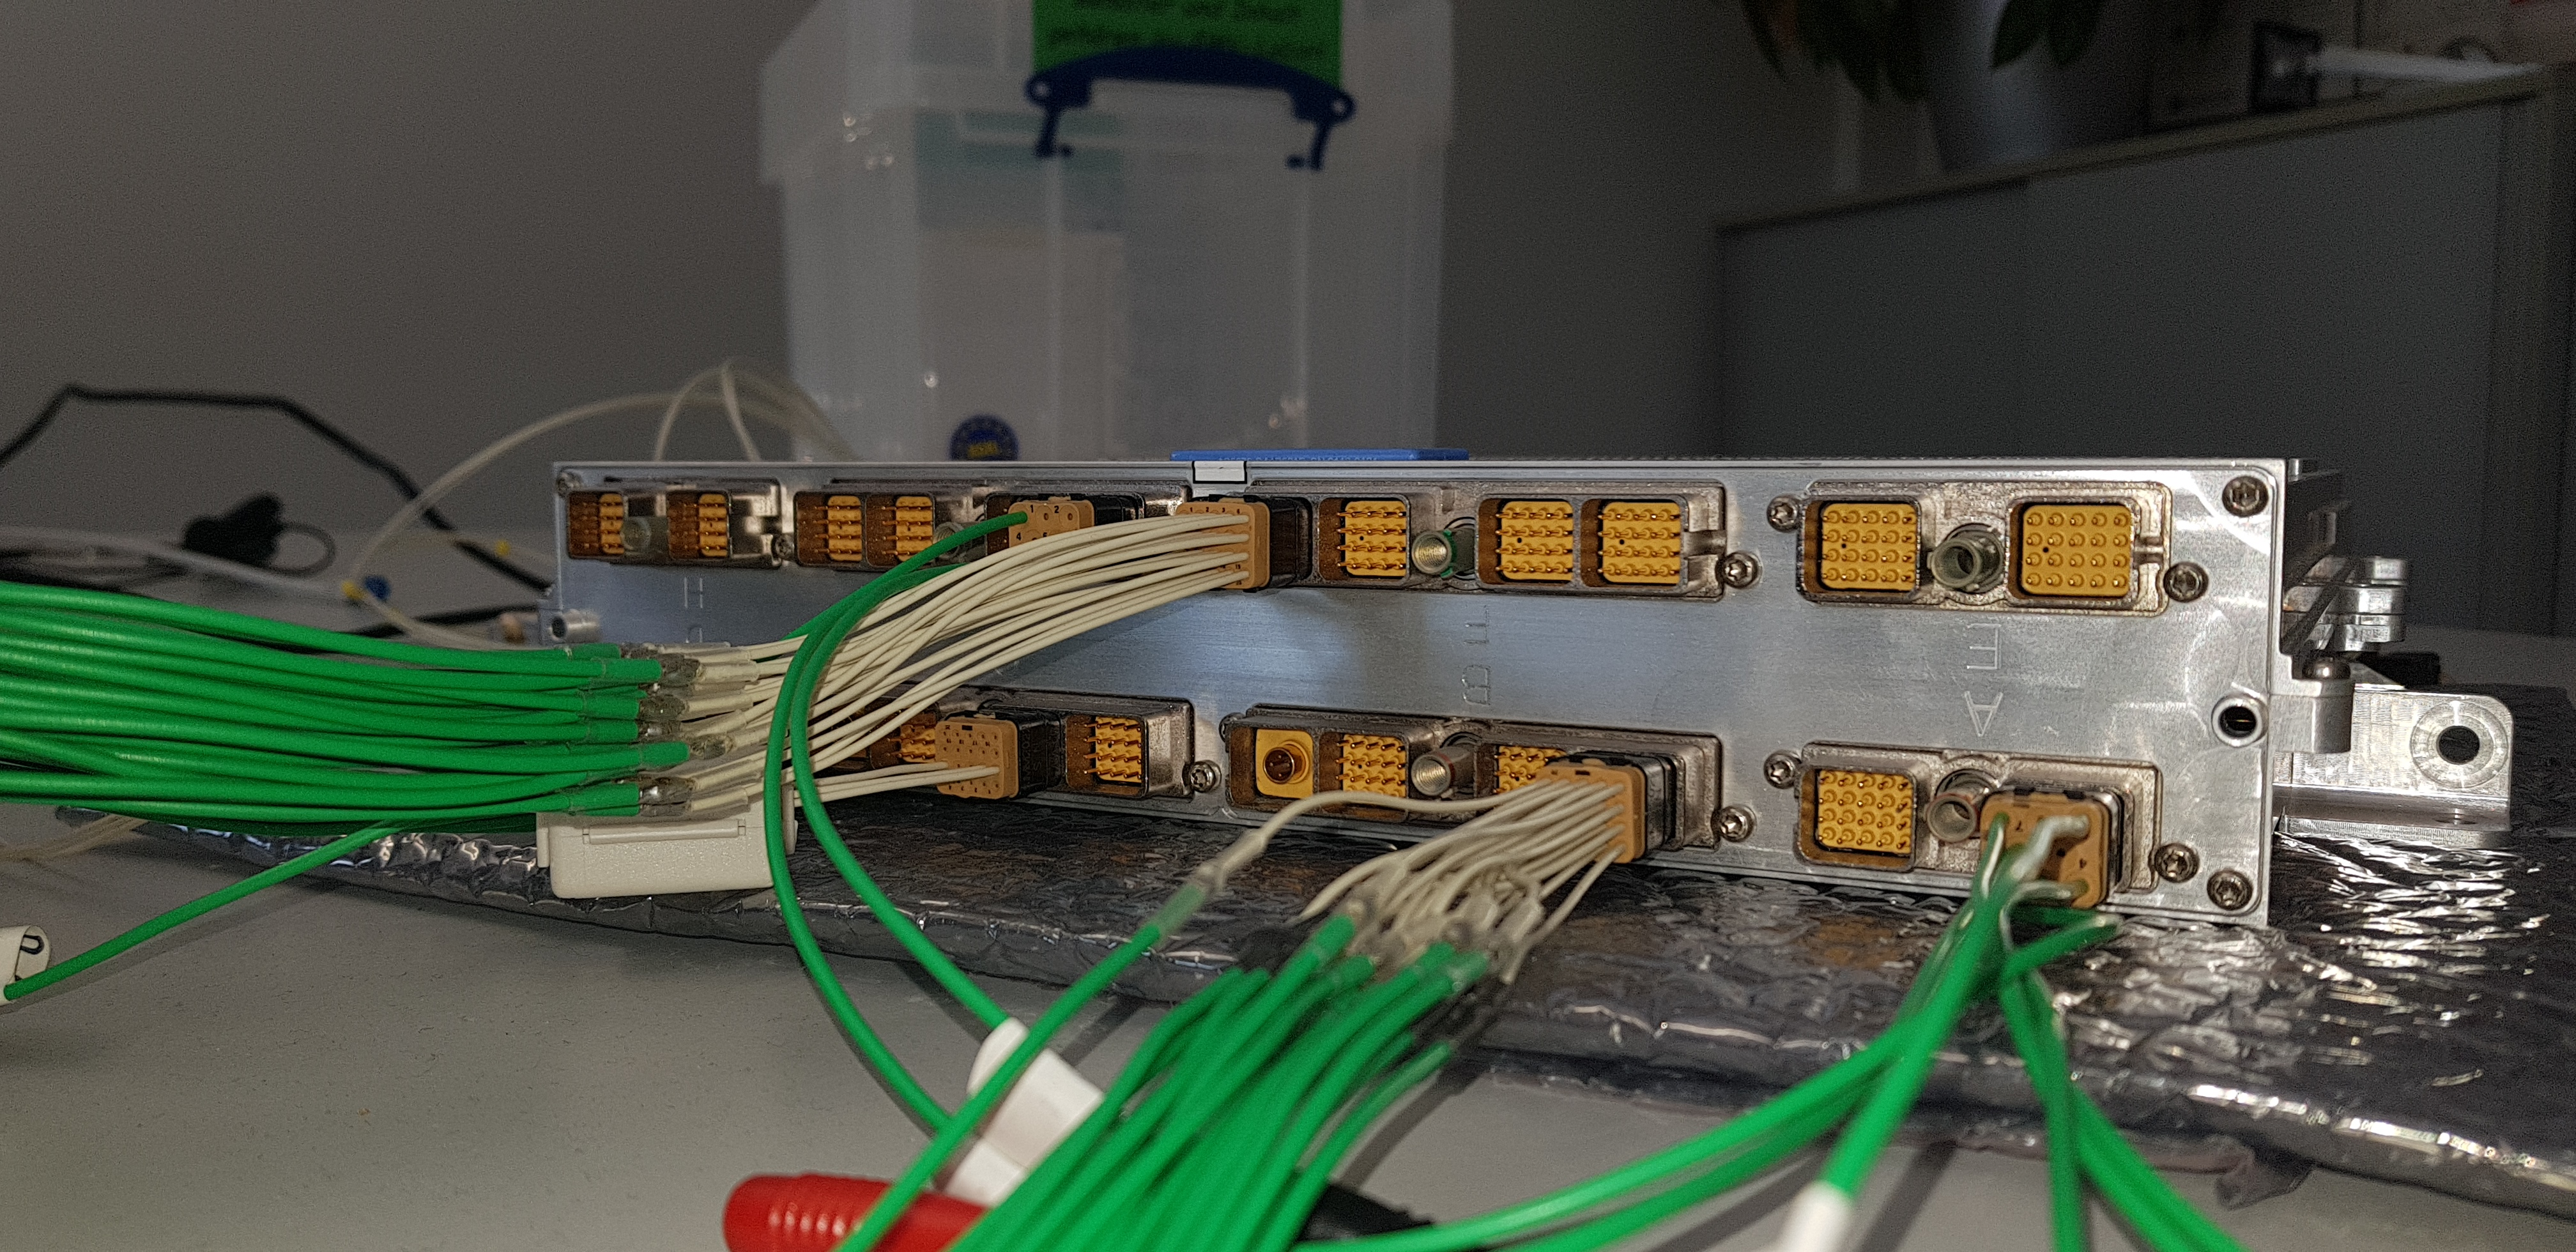
\includegraphics[width=\textwidth, height=0.5\textwidth]{graphics/crdc_1.png}
		\caption{RDC Type A Pins}
		\label{fig:crdc-pins}
	\end{minipage}
	\begin{minipage}{0.5\textwidth}
		\centering
		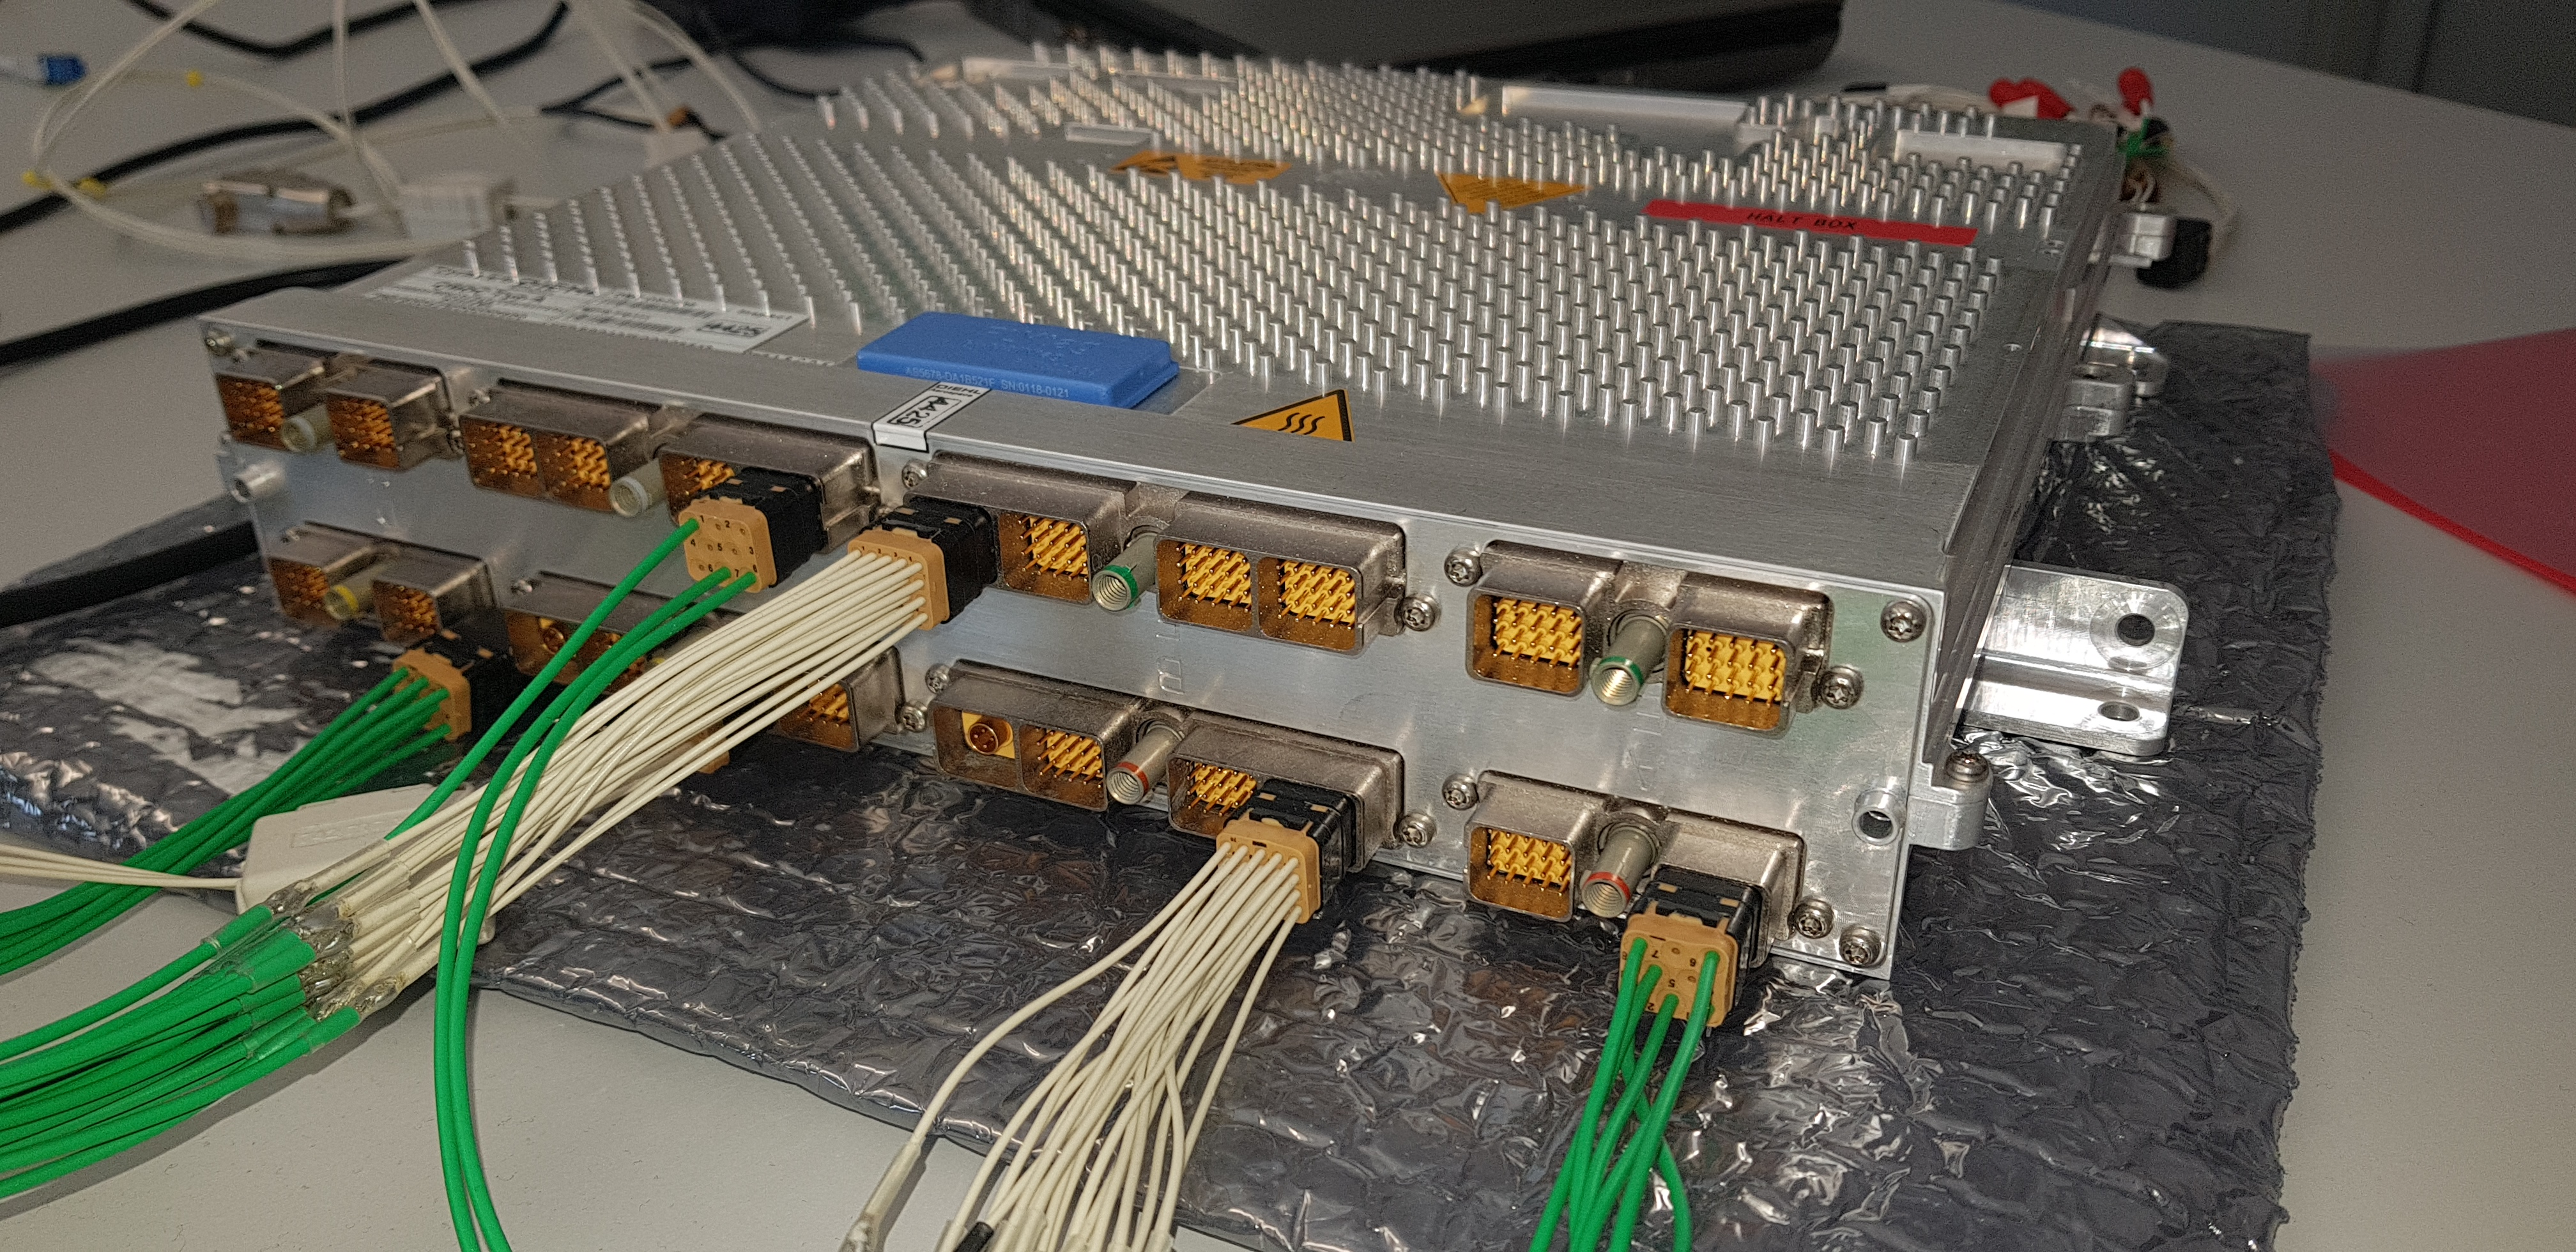
\includegraphics[width=\textwidth, height=0.5\textwidth]{graphics/crdc_2.png}
		\caption{RDC Type A}
		\label{fig:crdc_top}
	\end{minipage}
\end{figure}

Ein \ac{rdc} besteht aus einem Input/Output Interface um Verbindungen zu einem oder 
mehreren Input/Output Geräten und einem Netzwerk Interface, um eine Verbindung zu einem 
Fernprozessor zu ermöglichen.

%\section{Verbindung herstellen über das RS232-Interface}
%\label{sec:rs232-connection}

\section{Befehle Senden und Empfangen}
\label{sec:com-send-receive}

Um mit dem \ac{rdc} kommunizieren zu können werden Pins zu einem \ac{rs232}-Interface zur Verfügung gestellt. Mit Hilfe der Python-Bibliothek pySerial\footnote{\url{https://pyserial.readthedocs.io/en/latest/pyserial.html}} war es mir möglich ein Python Modul zu erstellen, dass sich um den Verbindungsaufbau, die Kommunikation und die Verbindungstrennung kümmert und kontrolliert. Mithilfe eines Threads konnte das Modul im Hintergrund auf den \ac{rs232}-Port hören ohne den Hauptteil des Programms dabei zu unterbrechen oder zu beeinträchtigen. Vorteil darin lag, dass der Workflow des Programms nur gestoppt wird wenn ein \ac{micbac}-Kommando an die \ac{uut} gesendet und eine Antwort erwartet wird. Dadurch war es mir möglich die Verbindung besser zu kontrollieren und Fehler wie \ac{zb} Datenverlust schneller zu erkennen. Des weiteren konnte ich so die Aufteilung der Programmstruktur besser einhalten und so einen besseren Überblick des Codes gewährleisten.

\subsection{Senden von MICBAC Commands}
\label{subsec:send-micbac}

Wie schon in Kapitel \ref{sec:com-send-receive} erwähnt werden zur Kommunikation sogenannte \ac{micbac}-Kommandos an die \ac{uut} geschickt. \ac{micbac}-Kommandos sind Befehle die über ein 32-Bit Mikrobussystem an die \ac{uut} gesendet werden und zur Steuerung und Abfrage von Information genutzt werden können. An jedem Pin eines \ac{rdc}s liegt ein anderes Interface an. Das bedeutet jedes Interface existiert in einem Gerät nur einmal. Nur der Typ des Interfaces kann gleich sein. Dadurch ist es möglich die Interface Typen in Python zu definieren und die Übersetzung der 32-Bit Befehle in die Typ-Definitionen zu implementieren.

\inputpython{scripts/send_micbac.py}{1}{15}{Send MICBAC Command}{lst:send-micbac}

Mithilfe von vorgefertigten Modulen von den Interface Typen aus einem anderen Projekt und den benötigten Adressinformationen, gespeichert in einer Tabelle, musste ich mich nur noch um das Einbinden der Module kümmern. Bevor ich die Module verwenden konnte musste der Code an manchen Stellen abgeändert und etwas um modelliert werden, da der Code in \citefield{Python}{note} 2 geschrieben wurde. In der eingelesen Testkonfiguration, die vom Tester erstellt wird, wird nur der Pin und der \ac{micbac}-Befehl angegeben was ein Problem darstellte, da der Pin nicht die benötigten Informationen enthielt. Durch  eingebettete Informationstabellen konnte ich in Hilfsmethoden dann die benötigten Informationen bestimmen, ein Objekt des benötigten Interface-Typen erstellen und den \ac{rs232}-Port registrieren. Am Ende musste ich nur noch den Befehl in der Interface-Typ-Instanz suchen und senden. Nachdem eine Antwort von der \ac{uut} empfangen wurde, wurden die Informationen an eine andere Methode übergeben und dort weiterverarbeitet.

\subsection{Empfangen von MICBAC Commands}
\label{subsec:receive-micbac}

\inputpython{scripts/receive_micbac.py}{1}{8}{Receive MICBAC Command}{lst:receive-micbac}

Nachdem Daten von der \ac{uut} empfangen wurde, werden diese an die Methode \textit{received\_msg()} übergeben. Da jeder Interface Typ unterschiedlich viele Datensätze als Antwort zurückschickt war es mir zum Ende hin nicht mehr möglich im Programm zu definieren wie viele Datensätze von einem Interface Typ benötigt werden um diese als eine vollständig gesendete Antwort zu bestimmen. Deshalb wurden erstmal alle Datensätze über einen vordefinierten Timer gesammelt und dann als Antwort in einer Liste gespeichert. Die Datensätze aus der Liste werden dann an die Methode \textit{start\_decode\_by\_msg()} übergeben. Dort werden sie in Adresse und Wert unterteilt und dann in der Interface-Typ-Instanz übersetzt und abgespeichert. Nach dem abspeicheren werden alle übersetzten Informationen aus der Interface-Typ-Instanz ausgelesen und zu einem lesbaren Text zusammengefügt. Der Text wird dann auf der \ac{gui} angezeigt und in einer Log-Datei abgespeichert.